\documentclass[tikz,border=8pt]{standalone}
\usetikzlibrary{calc}


\newcommand{\eradius}{3pt}
\newcommand{\blineouterradius}{7pt}
\newcommand{\blineinnerradius}{1pt}

\newcommand{\bline}[1]{%
    \draw[blue!80!black] (#1) circle (\blineouterradius);
    \fill[blue!80!black] (#1) circle (\blineinnerradius);
}


\begin{document}

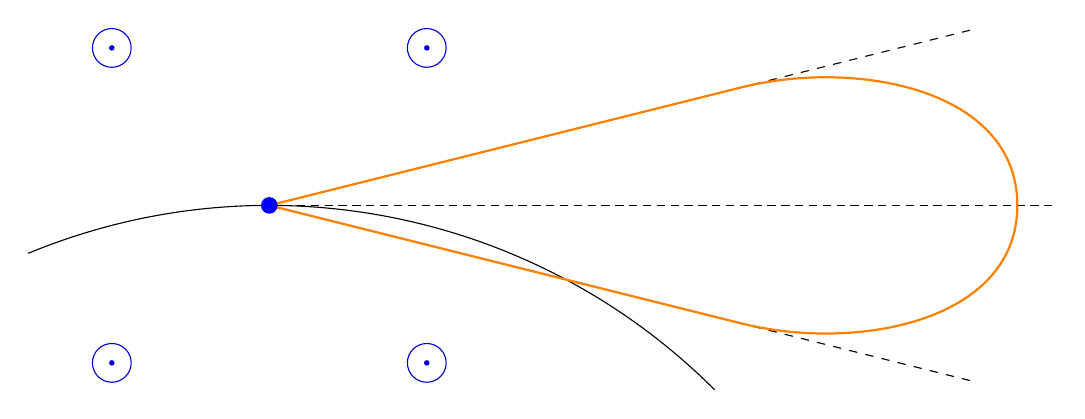
\begin{tikzpicture}

% gyration center at (4, -4), radius 8

% electron coordinates
\coordinate (e) at (4, 4);

% bline coordinates
\coordinate (B1) at (2, 2);
\coordinate (B2) at (2, 6);
\coordinate (B3) at (6, 6);
\coordinate (B4) at (6, 2);


% \draw[red] (4,-4) circle (8);
\draw (0.93853,3.39104) arc (112.5:45:8);
\draw[densely dashed] (e) -- (14, 4);
\draw[dashed] (e) -- (13, 6.25);
\draw[dashed] (e) -- (13, 1.75);
\draw[thick,orange] (e) -- (10, 5.5);
\draw[thick,orange] (e) -- (10, 2.5);
% \draw[orange] (10, 5.5) to [out=14, in=-14] (10, 2.5);
\draw[thick,orange] (10, 5.5) to [out=14, in=90] (13.5, 4) to [out=-90, in=-14] (10, 2.5);
% \draw[orange] (10, 5.5) arc (14:-14:6);
\fill[blue] (e) circle (\eradius);
\foreach \bcoord in {B1, B2, B3, B4}
    \bline{\bcoord};

\end{tikzpicture}

\end{document}
